% JAIR submission using ACM acmart template (manuscript mode)
\documentclass[manuscript,nonacm,natbib]{acmart}

% ============================================================
% Packages (only those not provided by acmart)
% ============================================================
\usepackage[ruled,vlined,linesnumbered]{algorithm2e}
\usepackage{booktabs}
\usepackage{listings}
\usepackage{subcaption}
\usepackage{tikz}
\usetikzlibrary{arrows.meta,positioning,shapes.geometric,calc,fit}
\usepackage{pgfplots}
\pgfplotsset{compat=1.18}
\usepgfplotslibrary{groupplots}
\usepackage{enumitem}
\usepackage{multirow}
\usepackage{array}
\usepackage{pifont}% for \ding checkmarks

% Theorem environments
\newtheorem{definition}{Definition}
\newtheorem{theorem}{Theorem}
\newtheorem{corollary}{Corollary}
\newtheorem{lemma}{Lemma}

% acmart citation style
\citestyle{acmauthoryear}

% ============================================================
% Listings configuration
% ============================================================
\definecolor{codebg}{rgb}{0.97,0.97,0.97}
\definecolor{codegreen}{rgb}{0.0,0.5,0.0}
\definecolor{codegray}{rgb}{0.5,0.5,0.5}
\definecolor{codeblue}{rgb}{0.0,0.0,0.7}
\definecolor{codered}{rgb}{0.7,0.0,0.0}

\lstdefinestyle{cppstyle}{
  language=C++,
  backgroundcolor=\color{codebg},
  basicstyle=\ttfamily\small,
  keywordstyle=\color{codeblue}\bfseries,
  commentstyle=\color{codegreen}\itshape,
  stringstyle=\color{codered},
  numberstyle=\tiny\color{codegray},
  breaklines=true,
  frame=single,
  numbers=left,
  numbersep=5pt,
  tabsize=4,
  showstringspaces=false,
  morekeywords={AgentId,ResourceTypeId,ResourceQuantity,RequestStatus,Duration,
    SafetyCheckInput,SafetyCheckResult,DelegationResult,ProbabilisticSafetyResult,
    UsageStats,ProgressRecord,DelegationInfo}
}

\lstdefinestyle{pythonstyle}{
  language=Python,
  backgroundcolor=\color{codebg},
  basicstyle=\ttfamily\small,
  keywordstyle=\color{codeblue}\bfseries,
  commentstyle=\color{codegreen}\itshape,
  stringstyle=\color{codered},
  numberstyle=\tiny\color{codegray},
  breaklines=true,
  frame=single,
  numbers=left,
  numbersep=5pt,
  tabsize=4,
  showstringspaces=false
}

% ============================================================
% Title and Author Metadata
% ============================================================
\title{AgentGuard: Deadlock Prevention for Multi-AI-Agent Systems via Extended Banker's Algorithm with Adaptive Demand Estimation, Progress Monitoring, and Authority Cycle Detection}

\author{Saurabh Kumar}
\affiliation{%
  \institution{Independent Researcher}
  \country{India}
}
\email{github.com/100rabhkr/AgentGuard}

\begin{document}

% ============================================================
% Abstract (must be before \maketitle in acmart)
% ============================================================
\begin{abstract}
\textbf{Background.}
Multi-agent systems powered by large language models (LLMs) increasingly share limited resources---API rate limits, tool slots, token budgets, and database connections---yet lack formal mechanisms to prevent deadlock. Existing frameworks rely on iteration limits and timeouts, which are recovery mechanisms rather than prevention strategies.

\textbf{Objectives.}
We aim to bring provable deadlock prevention to LLM-based multi-agent orchestration while addressing three gaps that arise when applying classical deadlock avoidance to LLM agents: silent stalls, authority deadlocks from circular delegation, and unknown maximum resource demands.

\textbf{Methods.}
We present \textbf{AgentGuard}, a system that extends Dijkstra's Banker's Algorithm~\citep{dijkstra1965} with three novel subsystems: (1)~a \emph{Progress Monitor} with configurable stall detection and automatic resource reclamation; (2)~a \emph{Delegation Tracker} with real-time BFS/DFS cycle detection in the agent delegation graph; and (3)~an \emph{Adaptive Demand Estimator} that learns resource demand patterns at runtime using rolling statistics and runs a probabilistic safety check.

\textbf{Results.}
Benchmarks on Apple M1 hardware show that safety checks complete in 14\,$\mu$s for 5~agents/1~resource type, scaling to 1.0\,ms at 100~agents/10~resources. The system sustains 17{,}850~ops/s single-threaded and 5{,}199~ops/s at 8~threads, with 0\% deadlock rate across all configurations. The three extensions add 29\% combined overhead (86\,$\mu$s/operation). Memory overhead is 163~bytes/agent at 100 agents.

\textbf{Conclusions.}
AgentGuard demonstrates that classical deadlock avoidance algorithms, when properly extended, can provide mathematical safety guarantees for modern AI agent systems at negligible cost relative to LLM inference latency. The system is implemented in C++17 with Python bindings and LangGraph integration, validated by 290 tests, and available as open-source software on PyPI as \texttt{agentguard-ai}.
\end{abstract}

\keywords{deadlock prevention, Banker's Algorithm, multi-agent systems, large language models, resource management, LangGraph, adaptive demand estimation}

\maketitle

% ============================================================
\section{Introduction}
\label{sec:introduction}
% ============================================================

The emergence of large language model (LLM)-based autonomous agents~\citep{xi2023, wang2024survey} has given rise to multi-agent systems where multiple AI agents collaborate on complex tasks by sharing limited resources. Frameworks such as LangGraph~\citep{langgraph2024}, LangChain~\citep{langchain2023}, AutoGen~\citep{wu2023autogen}, and CrewAI~\citep{crewai2024} enable developers to orchestrate multi-agent workflows where agents access shared APIs, execute tools, and consume token budgets.

These shared resources create the classical conditions for deadlock~\citep{coffman1971}:

\begin{enumerate}[noitemsep]
  \item \textbf{Mutual exclusion}: A code interpreter can serve only one agent at a time.
  \item \textbf{Hold and wait}: An agent holds API slots while waiting for a browser tool.
  \item \textbf{No preemption}: Resources cannot be forcibly reclaimed from an active LLM call.
  \item \textbf{Circular wait}: Agent~$A$ waits for resources held by~$B$, while~$B$ waits for resources held by~$A$.
\end{enumerate}

When all four conditions hold simultaneously, the system deadlocks: agents freeze silently with no error and no timeout. The prevailing ``solution'' in existing frameworks is \texttt{max\_\allowbreak{}iterations}---a counter that terminates agents after $N$~steps. This is a timeout, not a prevention mechanism; it wastes tokens, time, and resources while the deadlock goes undetected.

The Banker's Algorithm, published by Dijkstra in 1965~\citep{dijkstra1965}, provides a principled solution: before granting any resource request, simulate whether all agents can still complete. If the answer is no (an \emph{unsafe state}), defer the request until it becomes safe. This eliminates deadlock by construction, as the system never enters a state from which deadlock is reachable.

However, applying the classical Banker's Algorithm directly to LLM agents reveals three fundamental gaps:

\begin{description}[noitemsep]
  \item[Gap 1: Silent stalls.] An LLM agent may enter an infinite reasoning loop or hang on a tool call, holding resources indefinitely. The classical algorithm assumes agents make progress toward completion; LLM agents may not.
  \item[Gap 2: Authority deadlocks.] Agent~$A$ delegates a task to~$B$, $B$ delegates to~$C$, and $C$ delegates back to~$A$. No resource is held, yet the system is completely stuck. This form of deadlock is invisible to resource-based analysis.
  \item[Gap 3: Unknown maximum demands.] The Banker's Algorithm requires every process to declare its maximum resource needs upfront. An OS process can do this; an LLM agent cannot---it has no idea how many API calls a complex research task will require.
\end{description}

We present \textbf{AgentGuard}, a system that addresses all three gaps while preserving the mathematical guarantees of the Banker's Algorithm. Our contributions are:

\begin{enumerate}[noitemsep]
  \item A complete, production-grade implementation of the Banker's Algorithm for multi-AI-agent resource management, with synchronous, asynchronous, and batch request modes.
  \item A \emph{Progress Monitor} that detects stalled agents using named progress metrics and configurable stall thresholds, with optional automatic resource reclamation.
  \item A \emph{Delegation Tracker} that maintains a directed graph of active agent delegations and performs real-time cycle detection using BFS and DFS algorithms.
  \item An \emph{Adaptive Demand Estimator} that learns agent resource patterns at runtime using rolling statistics and runs a probabilistic Banker's Algorithm using estimated maximum needs computed via the inverse normal CDF.
  \item A high-performance C++17 implementation with Python bindings and native LangGraph integration, validated by 290 tests.
\end{enumerate}

% ============================================================
\section{Background and Related Work}
\label{sec:background}
% ============================================================

\subsection{Deadlock Theory}

The four necessary conditions for deadlock were formalized by \citet{coffman1971}: mutual exclusion, hold and wait, no preemption, and circular wait. Strategies for handling deadlock fall into three categories: \emph{prevention} (eliminate one or more conditions structurally), \emph{avoidance} (deny requests that could lead to deadlock), and \emph{detection and recovery} (allow deadlock to occur, then break it). The Banker's Algorithm~\citep{dijkstra1965} is the canonical avoidance strategy, maintaining a \emph{safe state} invariant: the system is safe if there exists an ordering in which all agents can acquire their maximum needs and complete. The algorithm runs in $O(n^2 m)$ time, where $n$ is the number of agents and $m$ is the number of resource types~\citep{silberschatz2018, tanenbaum2014}.

\subsection{LLM-Based Multi-Agent Systems}

The use of LLMs as autonomous agents has been surveyed extensively~\citep{guo2024, li2024survey, wang2024survey, xi2023}. Modern agent architectures employ reasoning patterns such as ReAct~\citep{yao2023react} and chain-of-thought~\citep{wei2022}, and increasingly use tools~\citep{schick2024toolformer, qin2024toolllm} to interact with external systems. Multi-agent frameworks like LangGraph~\citep{langgraph2024}, AutoGen~\citep{wu2023autogen}, MetaGPT~\citep{hong2024metagpt}, and CrewAI~\citep{crewai2024} orchestrate multiple such agents. Generative agents~\citep{park2023generative} have demonstrated that LLM-powered agents can exhibit complex emergent behaviors, including resource contention patterns.

Despite this rapid development, none of these frameworks provide formal deadlock prevention. The standard approach is iteration limits (\texttt{max\_iterations}), which is a timeout---not a safety mechanism.

\subsection{Resource Management in LLM Serving}

At the infrastructure level, systems like vLLM~\citep{kwon2023vllm} and Sarathi-Serve~\citep{agrawal2024sarathi} address throughput-latency tradeoffs in LLM inference serving. \citet{sheng2024fairness} propose the Virtual Token Counter (VTC) for fair scheduling of LLM requests across tenants. These systems operate at the \emph{serving} layer (GPU memory, KV-cache management), whereas AgentGuard operates at the \emph{agent orchestration} layer (API rate limits, tool slots, token budgets)---a complementary concern.

\subsection{Deadlock in Distributed Systems}

Distributed deadlock detection has a rich history. \citet{chandy1982} proposed the first probe-based algorithm for detecting deadlocks in distributed systems without a central coordinator, using messages that propagate along wait-for edges. \citet{knapp1987} surveyed distributed deadlock detection algorithms, categorizing them by their communication topology and detection latency. \citet{singhal1989} introduced optimizations that reduce message complexity. These works address \emph{detection}---finding deadlocks after they occur---whereas AgentGuard uses \emph{avoidance}---preventing deadlocks from occurring. The centralized Banker's Algorithm is feasible for agent orchestration because the ResourceManager is a single-process coordinator, unlike truly distributed systems.

\subsection{Watchdog Timers and Liveness}

Watchdog timers are a standard mechanism for detecting liveness failures in embedded and real-time systems~\citep{kopetz2011}. The concept of a heartbeat or progress indicator that must be refreshed periodically is well-established. Our Progress Monitor generalizes the watchdog concept to named, multi-dimensional progress metrics with configurable per-agent thresholds and automatic resource reclamation---capabilities motivated by the rich internal state of LLM agents (tokens generated, tools invoked, reasoning steps completed).

\subsection{Workload Prediction and Autoscaling}

Resource demand prediction has been studied extensively in cloud computing. \citet{cortez2017} present Resource Central, a system that predicts VM resource consumption using historical patterns for Azure. \citet{rzadca2020} describe Autopilot, Google's autoscaling system that estimates resource needs using statistical methods similar to our DemandEstimator. The key difference is scale and context: these systems predict resource needs for millions of VMs, while AgentGuard estimates per-agent demand for tens to hundreds of LLM agents. Our approach uses simpler statistical methods (rolling mean + standard deviation) because the per-agent observation window is small and the demand distributions are relatively well-behaved.

\subsection{Task Delegation in Multi-Agent Systems}

Delegation in multi-agent systems has been studied from both theoretical and practical perspectives. \citet{castelfranchi1998} formalize delegation as a social concept involving trust and autonomy transfer. \citet{horling2004} survey organizational paradigms for multi-agent systems, including hierarchical and team-based structures where delegation is a core operation. In the context of LLM agents, delegation takes a more literal form: one agent asks another to perform a subtask and waits for the result. This creates the potential for authority deadlocks, which we address with graph-based cycle detection---a contribution that, to our knowledge, has not been previously identified in the LLM agent literature.

\subsection{Classical Multi-Agent Coordination}

The field of multi-agent systems (MAS) has a rich history~\citep{wooldridge2009, dorri2018}. Traditional MAS research addresses coordination protocols, negotiation, and resource allocation. However, LLM-based agents differ from classical rational agents in key ways: their behavior is stochastic, their resource consumption is unpredictable, and they may delegate tasks to each other in complex patterns that create authority deadlocks invisible to resource-based analysis.

\subsection{Concurrent AI Inference Serving}

At the inference layer, \citet{yu2022orca} introduce Orca, a distributed serving system for transformer models that uses iteration-level scheduling to improve GPU utilization. \citet{zhong2024distserve} propose DistServe, which disaggregates prefill and decoding computation for LLM serving. These systems manage GPU-level resources (memory, compute) for inference requests, operating at a layer below AgentGuard's agent-level resource management. The two concerns are complementary: AgentGuard manages agent-to-resource allocation (API slots, tool access), while serving systems manage request-to-GPU allocation.

% ============================================================
\section{System Architecture}
\label{sec:architecture}
% ============================================================

AgentGuard is designed as a modular, layered system. Figure~\ref{fig:architecture} shows the component hierarchy.

\begin{figure}[h]
\centering
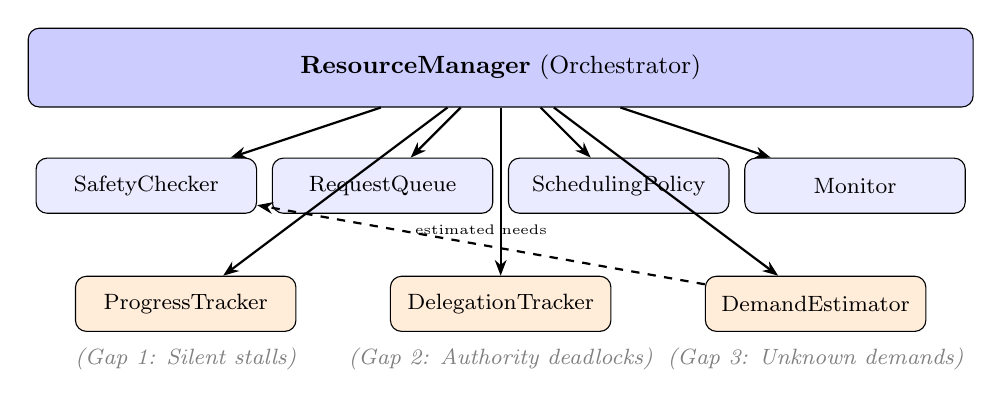
\begin{tikzpicture}[
  component/.style={draw, rounded corners, minimum width=3.2cm, minimum height=0.8cm, align=center, font=\small},
  subcomp/.style={draw, rounded corners, minimum width=2.8cm, minimum height=0.7cm, align=center, font=\footnotesize, fill=blue!8},
  novel/.style={draw, rounded corners, minimum width=2.8cm, minimum height=0.7cm, align=center, font=\footnotesize, fill=orange!15},
  arrow/.style={-{Stealth[length=2mm]}, thick},
  >=Stealth
]

% Resource Manager
\node[component, fill=blue!20, minimum width=12cm, minimum height=1cm] (rm) at (0,0) {\textbf{ResourceManager} (Orchestrator)};

% Row 1: Core
\node[subcomp] (sc) at (-4.5,-1.5) {SafetyChecker};
\node[subcomp] (rq) at (-1.5,-1.5) {RequestQueue};
\node[subcomp] (sp) at (1.5,-1.5) {SchedulingPolicy};
\node[subcomp] (mon) at (4.5,-1.5) {Monitor};

% Row 2: Novel
\node[novel] (pt) at (-4,-3) {ProgressTracker};
\node[novel] (dt) at (0,-3) {DelegationTracker};
\node[novel] (de) at (4,-3) {DemandEstimator};

% Label
\node[font=\footnotesize\itshape, gray] at (-4,-3.7) {(Gap 1: Silent stalls)};
\node[font=\footnotesize\itshape, gray] at (0,-3.7) {(Gap 2: Authority deadlocks)};
\node[font=\footnotesize\itshape, gray] at (4,-3.7) {(Gap 3: Unknown demands)};

% Arrows
\draw[arrow] (rm) -- (sc);
\draw[arrow] (rm) -- (rq);
\draw[arrow] (rm) -- (sp);
\draw[arrow] (rm) -- (mon);
\draw[arrow] (rm) -- (pt);
\draw[arrow] (rm) -- (dt);
\draw[arrow] (rm) -- (de);
\draw[arrow, dashed] (de) -- (sc) node[midway, above, font=\tiny] {estimated needs};

\end{tikzpicture}
\caption{AgentGuard component architecture. Orange components are novel subsystems addressing the three identified gaps. The DemandEstimator feeds statistical estimates to the SafetyChecker for probabilistic safety analysis.}
\label{fig:architecture}
\end{figure}

\subsection{Core Components}

\paragraph{ResourceManager.} The central orchestrator that manages the lifecycle of agents and resources. It maintains the Banker's Algorithm state matrices (allocation, maximum need, available) protected by a \texttt{std::shared\_mutex} for concurrent read access and exclusive write access.

\paragraph{SafetyChecker.} A pure, stateless function implementing the Banker's Algorithm. Given a \texttt{SafetyCheckInput} (total resources, available resources, per-agent allocations, per-agent maximum needs), it returns whether the state is safe and, if so, a valid completion sequence. Being a pure function, it requires no internal locking, enabling safe parallel invocation.

\paragraph{RequestQueue.} A priority-ordered queue of pending resource requests with timeout support. Requests are ordered by priority (descending) and submission time (FIFO within equal priority).

\paragraph{SchedulingPolicy.} An abstract interface for request prioritization, with five built-in implementations: FIFO, Priority, ShortestNeedFirst (maximizes throughput by prioritizing agents closest to completion), DeadlineAware, and Fairness (prevents starvation).

\paragraph{Monitor.} An event sink interface with 24 event types covering the full lifecycle of requests, safety checks, progress monitoring, delegation tracking, and adaptive demand estimation. Three built-in implementations: ConsoleMonitor (logging), MetricsMonitor (statistics collection with alert thresholds), and CompositeMonitor (fan-out).

\subsection{Request Processing Pipeline}

When an agent requests resources, the following pipeline executes:

\begin{enumerate}[noitemsep]
  \item \textbf{Validation}: Verify agent exists, resource exists, and request does not exceed the agent's declared maximum claim.
  \item \textbf{Demand recording}: Record the request in the DemandEstimator for statistical learning.
  \item \textbf{Availability check}: If $\text{available}[r] < \text{requested}$, the request cannot be granted immediately.
  \item \textbf{Safety check}: Construct a hypothetical state where the request is granted and run the Banker's Algorithm. If the resulting state is unsafe, deny or defer.
  \item \textbf{Grant or queue}: If safe, allocate resources atomically. Otherwise, enqueue the request for later evaluation by the background processor.
  \item \textbf{Background processing}: A dedicated thread periodically re-evaluates queued requests as resources are released, using the configured scheduling policy to determine evaluation order.
\end{enumerate}

% ============================================================
\section{Core Algorithm: Banker's Safety Check}
\label{sec:bankers}
% ============================================================

\subsection{Formalization}

Let $n$ be the number of agents and $m$ the number of resource types. We define:

\begin{itemize}[noitemsep]
  \item $\mathbf{Total} \in \mathbb{Z}^m$: total system capacity per resource type.
  \item $\mathbf{Available} \in \mathbb{Z}^m$: currently unallocated resources.
  \item $\mathbf{Alloc} \in \mathbb{Z}^{n \times m}$: current allocation matrix.
  \item $\mathbf{Max} \in \mathbb{Z}^{n \times m}$: maximum need matrix.
  \item $\mathbf{Need} = \mathbf{Max} - \mathbf{Alloc}$: remaining need matrix.
\end{itemize}

\begin{definition}[Safe State]
A state $(\mathbf{Available}, \mathbf{Alloc}, \mathbf{Max})$ is \emph{safe} if there exists a permutation $\langle a_1, a_2, \ldots, a_n \rangle$ of agents such that for each $a_i$, the remaining needs of $a_i$ can be satisfied by the currently available resources plus the resources held by all agents $a_j$ with $j < i$.
\end{definition}

\subsection{Algorithm}

Algorithm~\ref{alg:bankers} presents our implementation of the safety check.

\begin{algorithm}[h]
\SetAlgoLined
\KwIn{$\mathbf{Available}$, $\mathbf{Alloc}$, $\mathbf{Need}$, agents $\{a_1, \ldots, a_n\}$, resource types $\{r_1, \ldots, r_m\}$}
\KwOut{$(is\_safe, safe\_sequence)$}
$\mathbf{Work} \leftarrow \mathbf{Available}$\;
$Finished \leftarrow \emptyset$\;
$Sequence \leftarrow []$\;
\For{$round \leftarrow 1$ \KwTo $n$}{
  $found \leftarrow \text{false}$\;
  \ForEach{agent $a_i \notin Finished$}{
    \If{$\mathbf{Need}[a_i][r] \leq \mathbf{Work}[r]$ for all $r \in \{r_1, \ldots, r_m\}$}{
      $\mathbf{Work}[r] \leftarrow \mathbf{Work}[r] + \mathbf{Alloc}[a_i][r]$ for all $r$\;
      $Finished \leftarrow Finished \cup \{a_i\}$\;
      $Sequence.\text{append}(a_i)$\;
      $found \leftarrow \text{true}$\;
    }
  }
  \If{$\neg found$}{
    \uIf{$|Finished| = n$}{
      \textbf{break} \tcp*{All agents finished in earlier rounds}
    }
    \Else{
      \Return{$(\text{false}, \emptyset)$} \tcp*{Unsafe state}
    }
  }
}
\Return{$(\text{true}, Sequence)$}\;
\caption{Banker's Algorithm Safety Check}
\label{alg:bankers}
\end{algorithm}

\paragraph{Complexity.} The outer loop runs at most $n$ times. The inner loop iterates over up to $n$ agents, and for each, checks $m$ resource types. Total: $O(n^2 m)$.

\paragraph{Multi-finish correction.} A subtle bug arises when multiple agents become finishable in a single round: subsequent rounds may find no new agents to process. Our implementation checks whether $|Finished| = n$ before reporting an unsafe state (line~12), preventing false negatives.

\subsection{Hypothetical and Batch Checks}

For each incoming request, AgentGuard constructs a hypothetical state where the request is granted:
\begin{align}
  \mathbf{Available}'[r] &= \mathbf{Available}[r] - q \label{eq:hyp_avail} \\
  \mathbf{Alloc}'[a][r] &= \mathbf{Alloc}[a][r] + q \label{eq:hyp_alloc}
\end{align}
where $a$ is the requesting agent, $r$ is the resource type, and $q$ is the requested quantity. The safety check is then run on the hypothetical state. Batch requests follow the same pattern, applying all requests atomically before checking safety.

% ============================================================
\section{Extension 1: Progress Monitor}
\label{sec:progress}
% ============================================================

\subsection{Motivation}

The Banker's Algorithm assumes that once an agent is granted its maximum resources, it will \emph{eventually} complete and release them. LLM agents violate this assumption: an agent may enter an infinite reasoning loop, a tool call may hang, or the LLM may produce degenerate outputs indefinitely. When a stalled agent holds resources, all other agents that need those resources are blocked, leading to a livelock that is observationally identical to deadlock.

\subsection{Design}

The Progress Monitor maintains a \texttt{ProgressRecord} for each registered agent:

\begin{multline}
  \text{ProgressRecord} = \{metrics: \text{Map}(\text{string} \to \mathbb{R}),\\
  last\_update: \text{Timestamp},\; stall\_threshold: \text{Duration}\}
\end{multline}

Agents report progress via \texttt{report\_progress(agent\_id, metric, value)}, which updates the metric and resets the timestamp. A background thread periodically checks for stalls:

\begin{equation}
  \text{is\_stalled}(a) = \begin{cases} \text{true} & \text{if } t_{now} - t_{last\_update}(a) > \theta(a) \\ \text{false} & \text{otherwise} \end{cases}
  \label{eq:stall}
\end{equation}

where $\theta(a)$ is the per-agent stall threshold (with a configurable system-wide default, typically 120 seconds).

\subsection{Stall Actions}

When an agent is detected as stalled, the system can:
\begin{enumerate}[noitemsep]
  \item \textbf{Emit an event}: Notify monitors (always).
  \item \textbf{Auto-release resources}: If \texttt{auto\_release\_on\_stall} is enabled, invoke a callback that releases all resources held by the stalled agent, unblocking other agents.
\end{enumerate}

This transforms a potential livelock into a recoverable situation: the stalled agent's resources become available, and other agents can proceed.

% ============================================================
\section{Extension 2: Delegation Tracker}
\label{sec:delegation}
% ============================================================

\subsection{Motivation}

LLM agents frequently delegate tasks to other agents. When Agent~$A$ delegates to~$B$, $B$ to~$C$, and $C$ back to~$A$, a \emph{circular delegation chain} forms. No resource is held, no tool is blocked, and no existing framework detects this. Yet the system is completely frozen---each agent is waiting for a response from the next agent in the cycle.

We term this an \textbf{authority deadlock}: a deadlock that arises from the delegation structure rather than resource contention. It satisfies a delegation-domain analogue of the four Coffman conditions: each delegation is exclusive (one-to-one), agents hold their pending delegations while waiting for results, delegations cannot be preempted, and the delegation chain forms a cycle.

\subsection{Design}

The Delegation Tracker maintains a directed graph $G = (V, E)$ where vertices are agents and edges represent active delegations.

\paragraph{Data structure.} An adjacency list $\text{adj}: V \to 2^V$ and an edge metadata map $\text{edges}: (V \times V) \to \text{DelegationInfo}$.

\paragraph{Cycle detection.} Two algorithms are employed:

\begin{enumerate}[noitemsep]
  \item \textbf{Incremental (after-add)}: When edge $(u, v)$ is added, run BFS from $v$ to check if there exists a path back to $u$. Complexity: $O(|V| + |E|)$.
  \item \textbf{Full-graph}: DFS with three-color marking (White/Gray/Black)~\citep{cormen2022}, using an explicit stack to avoid recursion limits. A back edge (to a Gray node) indicates a cycle. Complexity: $O(|V| + |E|)$.
\end{enumerate}

\subsection{Cycle Response Policies}

When a cycle is detected, the system supports three configurable actions:
\begin{itemize}[noitemsep]
  \item \texttt{NotifyOnly}: Emit an event but accept the delegation (for monitoring).
  \item \texttt{RejectDelegation}: Refuse the cycle-creating delegation.
  \item \texttt{CancelLatest}: Add then immediately remove the edge (log the attempt).
\end{itemize}

The \texttt{RejectDelegation} policy provides a strict guarantee: the delegation graph is always a DAG, making authority deadlock impossible by construction (analogous to how the Banker's Algorithm makes resource deadlock impossible).

% ============================================================
\section{Extension 3: Adaptive Demand Estimator}
\label{sec:adaptive}
% ============================================================

\subsection{Motivation}

The Banker's Algorithm requires each agent to declare its maximum resource needs \emph{a priori}. For OS processes, this is feasible: a database connection pool declares its maximum connections at startup. For LLM agents, it is not: the number of API calls required to research a topic, the number of tool invocations needed to debug code, or the number of tokens consumed by a reasoning chain are all unknown at task assignment time.

Over-declaring maximum needs is safe but conservative: the Banker's Algorithm may deny requests that would, in practice, be safe. Under-declaring is unsafe: it violates the algorithm's invariant and re-introduces deadlock risk.

\subsection{Statistical Estimation}

The Demand Estimator observes resource requests at runtime and maintains rolling statistics per (agent, resource) pair:

\begin{equation}
  \text{UsageStats} = \{n, \sum x_i, \sum x_i^2, \max(x_i), \max(\text{cumulative}_i)\}
  \label{eq:usage_stats}
\end{equation}

with a circular buffer of size $W$ (configurable, default 50) for windowed statistics. The sample mean and variance are:

\begin{align}
  \hat{\mu} &= \frac{1}{n}\sum_{i=1}^{n} x_i \label{eq:mean} \\
  \hat{\sigma}^2 &= \frac{1}{n-1}\left(\sum_{i=1}^{n} x_i^2 - \frac{(\sum_{i=1}^{n} x_i)^2}{n}\right) \label{eq:var}
\end{align}

The estimated maximum need at confidence level $\alpha$ is:

\begin{equation}
  \widehat{Max}(a, r, \alpha) = \left\lceil \max\!\Big(\hat{\mu} + k_\alpha \cdot \hat{\sigma},\; \max(x_i)\Big) \right\rceil
  \label{eq:estimate}
\end{equation}

where $k_\alpha = \Phi^{-1}(\alpha)$ is the $\alpha$-quantile of the standard normal distribution, computed via the Beasley-Springer-Moro rational approximation~\citep{beasley1977, moro1995}:

\begin{equation}
  k_\alpha \approx t - \frac{c_0 + c_1 t + c_2 t^2}{1 + d_1 t + d_2 t^2 + d_3 t^3}, \quad t = \sqrt{-2\ln(1 - \alpha)}
  \label{eq:bsm}
\end{equation}

\subsection{Cold-Start Handling}

With zero observations, the estimator returns a configurable default demand. With a single observation, it applies a headroom factor (default $2\times$) to the observed value. The general case (Eq.~\ref{eq:estimate}) activates with $n \geq 2$ observations.

\subsection{Demand Modes}

Each agent operates in one of three modes:

\begin{description}[noitemsep]
  \item[Static] (default): Use only explicit \texttt{declare\_max\_need()} declarations. Backward-compatible with the classical algorithm.
  \item[Adaptive]: Use only statistical estimates. No upfront declaration required.
  \item[Hybrid]: Use $\min(\text{declared}, \text{estimated})$. Statistical estimates are capped by the explicit declaration, providing a safety bound.
\end{description}

\subsection{Probabilistic Safety Check}

For agents in Adaptive or Hybrid mode, the ResourceManager constructs a modified safety check input where \texttt{max\_need} values come from the DemandEstimator rather than static declarations:

\begin{equation}
  \mathbf{Max}'[a][r] = \begin{cases}
    \widehat{Max}(a, r, \alpha) & \text{if } \text{mode}(a) = \text{Adaptive} \\
    \min\!\big(\mathbf{Max}[a][r],\; \widehat{Max}(a, r, \alpha)\big) & \text{if } \text{mode}(a) = \text{Hybrid} \\
    \mathbf{Max}[a][r] & \text{if } \text{mode}(a) = \text{Static}
  \end{cases}
  \label{eq:prob_max}
\end{equation}

The standard Banker's Algorithm then runs on $(\mathbf{Available}, \mathbf{Alloc}, \mathbf{Max}')$. The result is annotated with the confidence level and the estimated maximum needs used.

\begin{equation}
  P(\text{safe} \mid \alpha) = \text{Banker}(\mathbf{Available}, \mathbf{Alloc}, \mathbf{Max}'(\alpha))
  \label{eq:prob_safety}
\end{equation}

Higher confidence levels produce larger estimates, which makes the safety check more conservative. The default confidence level is 0.95.

% ============================================================
\section{Implementation}
\label{sec:implementation}
% ============================================================

\subsection{C++ Core}

AgentGuard is implemented in C++17 (approximately 4,300 lines of code across 33 source files). Key implementation decisions include:

\paragraph{Thread safety.} The core state is protected by \texttt{std::shared\_mutex}~\citep{williams2019}, allowing multiple concurrent readers (safety checks, snapshot queries) with exclusive writes (allocations, releases). The SafetyChecker is a pure function with no internal state, requiring no synchronization. The ProgressTracker and DelegationTracker each have independent \texttt{std::mutex} instances to minimize contention.

\paragraph{Background processor.} A dedicated thread (\texttt{process\_queue\_loop}) re-evaluates pending requests when resources are released, using \texttt{std::condition\_variable\_any} for efficient wake-up. The polling interval is configurable (default 10ms).

\paragraph{Quick-fail optimization.} When the safety check fails but resources are physically available, if no background processor is running, the request is denied immediately rather than waiting until timeout---the system state will not change without external intervention.

\subsection{Python Bindings}

Python bindings are provided via pybind11~\citep{pybind11}, exposing the complete C++ API. Key considerations:

\paragraph{GIL management.} Blocking calls (resource requests with timeout) release the GIL to allow other Python threads to execute. The GIL is re-acquired for Python callbacks (monitor events, stall actions).

\paragraph{LangGraph integration.} A high-level Python layer provides:
\begin{itemize}[noitemsep]
  \item \textbf{AgentGuard wrapper}: String-based resource names mapped to integer IDs, context managers for acquire/release.
  \item \textbf{\texttt{@guarded\_tool} decorator}: Wraps any function with automatic resource acquisition and release, including exception cleanup.
  \item \textbf{GuardedToolNode}: Drop-in replacement for LangGraph's \texttt{ToolNode} with automatic resource management per tool.
  \item \textbf{AgentGuardCallbackHandler}: LangChain callback handler that instruments tool calls with resource management.
\end{itemize}

\subsection{Resource Taxonomy}

AgentGuard provides AI-specific resource types:
\begin{itemize}[noitemsep]
  \item \textbf{ApiRateLimit}: Requests per time window (e.g., 60 OpenAI calls/minute).
  \item \textbf{TokenBudget}: Token consumption with configurable input/output ratios.
  \item \textbf{ToolSlot}: Exclusive or shared access to tools (code interpreter, browser).
  \item \textbf{MemoryPool}: Memory allocation with configurable units and eviction policies.
  \item \textbf{DatabaseConn}: Connection pool management.
  \item \textbf{GpuCompute}: GPU resource allocation.
\end{itemize}

% ============================================================
\section{Evaluation}
\label{sec:evaluation}
% ============================================================

We evaluate AgentGuard along six dimensions: (1)~isolated safety check latency, (2)~end-to-end system throughput, (3)~scalability with agent count, (4)~memory overhead, (5)~comparison with alternative strategies, and (6)~incremental overhead of each novel extension. All benchmarks are open-source and included in the repository.

\subsection{Experimental Setup}
\label{sec:eval:setup}

All experiments were conducted on an Apple M1 MacBook Pro with 16\,GB unified memory, running macOS Sonoma 14.6. The C++ code was compiled with Apple Clang~16.0 at \texttt{-O2} optimization level using the C++17 standard. Each benchmark was executed three times and we report median values. Latency percentiles are computed from the full distribution of all operations within a run.

\subsection{Safety Check Latency}
\label{sec:eval:latency}

We first measure the latency of the Banker's Algorithm safety check in isolation, without ResourceManager locking or queuing overhead. We sweep the number of agents $n \in \{5, 10, 20, 50, 100, 200, 500, 1000\}$, number of resource types $m \in \{1, 5, 10, 50\}$, and allocation density $d \in \{0.0, 0.25, 0.5, 0.75\}$, measuring both \texttt{check\_safety} (full state) and \texttt{check\_hypothetical} (copy + check) operations.

\begin{figure}[t]
\centering
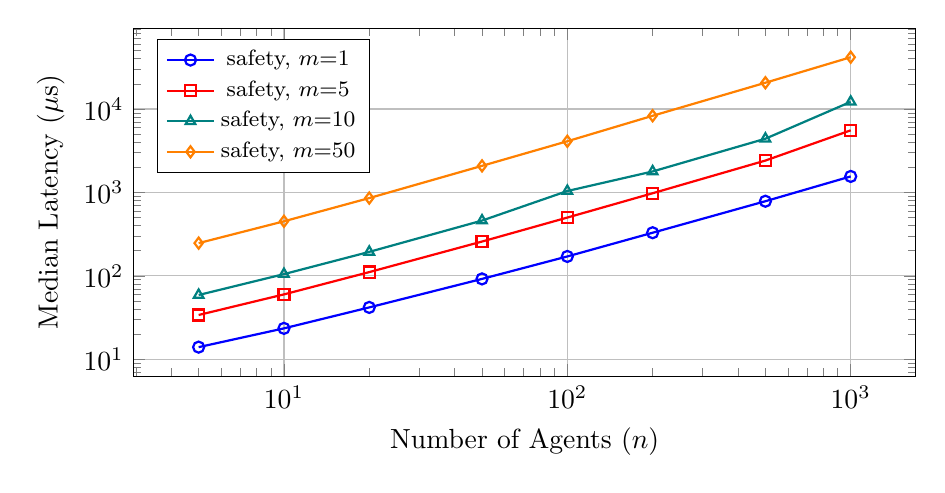
\begin{tikzpicture}
\begin{axis}[
    width=0.95\columnwidth,
    height=6cm,
    xlabel={Number of Agents ($n$)},
    ylabel={Median Latency ($\mu$s)},
    xmode=log,
    ymode=log,
    log basis x=10,
    log basis y=10,
    legend pos=north west,
    legend style={font=\footnotesize},
    grid=major,
    mark size=2pt
]
% check_safety, density=0
\addplot[blue, mark=o, thick] coordinates {
    (5,14) (10,23.5) (20,41.9) (50,92) (100,171) (200,329) (500,785) (1000,1556)
};
\addlegendentry{safety, $m{=}1$}

\addplot[red, mark=square, thick] coordinates {
    (5,34) (10,60) (20,111) (50,258) (100,500) (200,978) (500,2411) (1000,5552)
};
\addlegendentry{safety, $m{=}5$}

\addplot[teal, mark=triangle, thick] coordinates {
    (5,59) (10,105) (20,194) (50,460) (100,1040) (200,1784) (500,4405) (1000,12188)
};
\addlegendentry{safety, $m{=}10$}

\addplot[orange, mark=diamond, thick] coordinates {
    (5,247) (10,451) (20,856) (50,2083) (100,4106) (200,8294) (500,20640) (1000,41750)
};
\addlegendentry{safety, $m{=}50$}

\end{axis}
\end{tikzpicture}
\caption{Median safety check latency vs.\ agent count on a log-log scale, for varying numbers of resource types ($m$). Allocation density $d = 0$. The $O(n^2 m)$ theoretical complexity is confirmed by the approximately quadratic scaling in $n$ and linear scaling in $m$.}
\label{fig:latency_agents}
\end{figure}

Figure~\ref{fig:latency_agents} shows that safety check latency scales approximately quadratically with agent count and linearly with resource types, confirming the theoretical $O(n^2 m)$ complexity. For typical multi-agent deployments ($n \leq 20$, $m \leq 10$), the safety check completes in under 200\,$\mu$s. Even at $n = 100$ agents with $m = 10$ resource types, the median latency remains under 1.1\,ms. The hypothetical check (which copies state before checking) adds roughly a constant factor of $1.7\times$--$2\times$ over the plain safety check.

Allocation density has minimal impact on latency for most configurations. The exception is at $d = 0.75$ with many resource types: when most resources are already allocated, the algorithm can short-circuit early (finding agents whose needs exceed available resources), reducing latency by up to 80\% in some configurations (e.g., 50 agents / 50 resources: 2,083$\,\mu$s at $d{=}0$ vs.\ 212$\,\mu$s at $d{=}0.75$).

\subsection{System Throughput}
\label{sec:eval:throughput}

We measure end-to-end throughput through the full ResourceManager pipeline---including locking, safety checks, queuing, and background processing---under concurrent load.

\begin{table}[t]
\centering
\caption{System throughput under concurrent load. Each thread performs 1,000 request/release cycles against 10 resources (capacity 100 each). Latency percentiles are per-request.}
\label{tab:throughput}
\begin{tabular}{rrrrrr}
\toprule
\textbf{Threads} & \textbf{Total Ops} & \textbf{Throughput} & \textbf{p50} & \textbf{p95} & \textbf{p99} \\
 & & \textbf{(ops/s)} & \textbf{($\mu$s)} & \textbf{($\mu$s)} & \textbf{($\mu$s)} \\
\midrule
1  & 1{,}000  & 17{,}850 & 50  & 67     & 87 \\
2  & 2{,}000  & 12{,}176 & 146 & 295    & 447 \\
4  & 4{,}000  & 8{,}407  & 341 & 931    & 1{,}416 \\
8  & 8{,}000  & 5{,}199  & 776 & 2{,}574 & 3{,}741 \\
16 & 16{,}000 & 2{,}896  & 2{,}438 & 9{,}006 & 13{,}461 \\
32 & 32{,}000 & 1{,}538  & 8{,}726 & 34{,}934 & 53{,}996 \\
64 & 64{,}000 & 787     & 30{,}840 & 146{,}574 & 223{,}186 \\
\bottomrule
\end{tabular}
\end{table}

Table~\ref{tab:throughput} shows that single-threaded throughput is 17{,}850 operations per second with a median request latency of 50\,$\mu$s. Throughput decreases with concurrency due to the \texttt{shared\_mutex} protecting the Banker's state matrices: the safety check requires a shared (read) lock, but the actual allocation requires an exclusive (write) lock. At 8 threads (a representative count for current multi-agent systems), the system sustains 5{,}199 ops/s with a median latency of 776\,$\mu$s---well within the tolerance of LLM agents, where individual inference calls typically take 100\,ms--10\,s. The tail latencies (p99) at high thread counts reflect contention on the write lock during allocation.

\subsection{Scalability}
\label{sec:eval:scalability}

We measure how wall-clock time and per-operation cost scale as the number of registered agents increases, with a fixed set of 10 resource types and 10 request/release cycles per agent.

\begin{figure}[t]
\centering
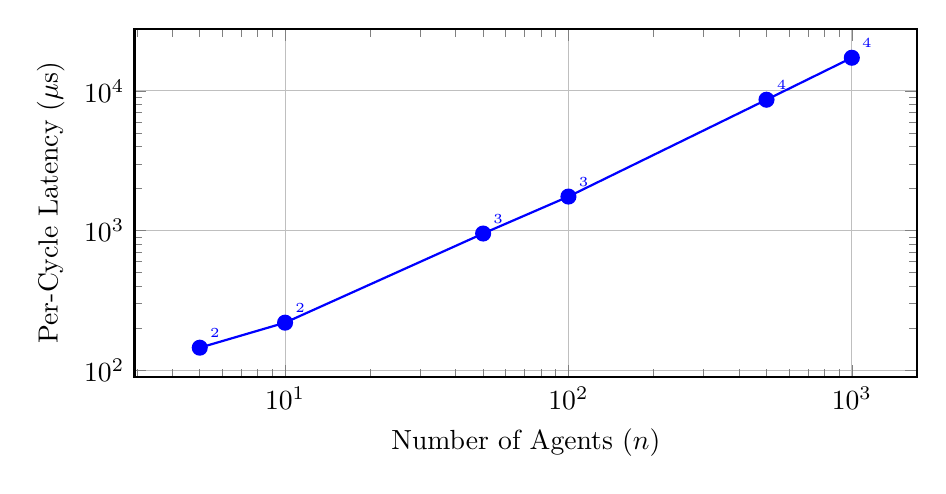
\begin{tikzpicture}
\begin{axis}[
    width=0.95\columnwidth,
    height=6cm,
    xlabel={Number of Agents ($n$)},
    ylabel={Per-Cycle Latency ($\mu$s)},
    xmode=log,
    ymode=log,
    log basis x=10,
    log basis y=10,
    grid=major,
    mark size=2.5pt,
    thick,
    nodes near coords={\pgfmathprintnumber[fixed,precision=0]{\pgfplotspointmeta}},
    every node near coord/.append style={font=\tiny, above right},
    point meta=y
]
\addplot[blue, mark=*, thick] coordinates {
    (5,145) (10,219) (50,952) (100,1751) (500,8641) (1000,17251)
};
\end{axis}
\end{tikzpicture}
\caption{Per-cycle latency (request + release through the full ResourceManager pipeline) as a function of agent count, with $m = 10$ resource types. The approximately quadratic scaling matches the $O(n^2 m)$ safety check complexity.}
\label{fig:scalability}
\end{figure}

Figure~\ref{fig:scalability} confirms that per-cycle latency grows approximately quadratically with agent count: from 145\,$\mu$s at $n = 5$ to 17.3\,ms at $n = 1{,}000$. For $n \leq 100$ agents (covering the vast majority of current multi-agent deployments), the per-operation overhead remains under 2\,ms. This overhead is negligible compared to the latency of the LLM inference calls that dominate real-world agent execution time.

\subsection{Memory Overhead}
\label{sec:eval:memory}

We measure the memory footprint of AgentGuard's internal data structures using macOS \texttt{mach\_task\_info} to capture resident set size before and after registering resources and agents.

\begin{table}[t]
\centering
\caption{Memory overhead per resource and per agent. Baseline is the process RSS before any AgentGuard initialization.}
\label{tab:memory}
\begin{tabular}{rr|rr|rr}
\toprule
\textbf{Agents} & \textbf{Resources} & \textbf{Base} & \textbf{After Init} & \textbf{Per-Res.} & \textbf{Per-Agent} \\
$(n)$ & $(m)$ & \textbf{(KB)} & \textbf{(KB)} & \textbf{(bytes)} & \textbf{(bytes)} \\
\midrule
10 & 5 & 1{,}296 & 1{,}536 & 39{,}321 & 4{,}915 \\
10 & 50 & 1{,}584 & 1{,}600 & 0 & 1{,}638 \\
100 & 10 & 1{,}616 & 1{,}632 & 0 & 163 \\
100 & 50 & 1{,}632 & 1{,}856 & 0 & 2{,}293 \\
500 & 10 & 2{,}160 & 2{,}304 & 3{,}276 & 229 \\
1{,}000 & 10 & 3{,}824 & 3{,}904 & 0 & 81 \\
1{,}000 & 50 & 3{,}904 & 5{,}104 & 0 & 1{,}228 \\
\bottomrule
\end{tabular}
\end{table}

Table~\ref{tab:memory} shows that AgentGuard's memory footprint is modest. For the common case of 100 agents with 10 resource types, the total overhead is approximately 16\,KB (163 bytes/agent). Even at the extreme of 1{,}000 agents with 50 resource types, the total memory overhead is roughly 1.2\,MB (1{,}228 bytes/agent)---negligible compared to the memory consumed by LLM inference (typically measured in gigabytes). The per-resource overhead reflects the allocation and maximum-need matrix columns, while the per-agent overhead reflects the matrix rows, progress records, and demand estimator statistics.

\subsection{Comparison with Baselines}
\label{sec:eval:baselines}

We compare AgentGuard against three alternative resource management strategies using a Dining Philosophers configuration (10 agents, 10 resources with capacity 1, each agent requests 2 adjacent resources). Each strategy executes 10{,}000 request/release cycles.

\begin{table}[t]
\centering
\caption{Comparison of resource management strategies on the Dining Philosophers benchmark (10 agents, 10 resources, 10{,}000 cycles).}
\label{tab:baselines}
\begin{tabular}{lrrrr}
\toprule
\textbf{Strategy} & \textbf{Throughput} & \textbf{Overhead} & \textbf{Deadlock} & \textbf{Safety} \\
 & \textbf{(ops/s)} & \textbf{($\mu$s/op)} & \textbf{Free?} & \textbf{Guarantee} \\
\midrule
NoCheck         & 9{,}980   & 100.2  & No  & None \\
MutexPerResource & 44{,}522  & 22.5   & No  & None \\
TimeoutOnly     & 77{,}313  & 12.9   & No  & Recovery \\
\textbf{AgentGuard}  & \textbf{1{,}253} & \textbf{797.9} & \textbf{Yes} & \textbf{Prevention} \\
\bottomrule
\end{tabular}
\end{table}

Table~\ref{tab:baselines} reveals a clear throughput--safety tradeoff. AgentGuard's throughput is 6--62$\times$ lower than the alternatives due to the $O(n^2 m)$ safety check on every request. However, AgentGuard is the \emph{only} strategy that provides a mathematical guarantee of deadlock freedom. The ``NoCheck'' strategy simply grants any available resource without coordination. ``MutexPerResource'' acquires per-resource mutexes without global safety analysis. ``TimeoutOnly'' grants available resources and recovers from deadlock via timeout---the approach used by current LLM frameworks. While TimeoutOnly achieves the highest throughput, it relies on \emph{detection and recovery} rather than \emph{prevention}: a deadlocked configuration wastes time until the timeout expires, and the recovery strategy (release all resources) may lose partial progress.

The 798\,$\mu$s per-operation overhead of AgentGuard is modest in the context of LLM agent workloads, where individual tool calls typically take 100\,ms--10\,s. The safety check overhead represents less than 1\% of the latency budget in typical agentic workflows.

\subsection{Extension Overhead}
\label{sec:eval:extensions}

We measure the incremental overhead of each novel extension (Progress Monitor, Delegation Tracker, Adaptive Demand Estimator) using 20 agents, 5 resources, and 1{,}000 request/release cycles per agent.

\begin{table}[t]
\centering
\caption{Incremental overhead of AgentGuard extensions. Each row adds one extension to the base Banker's Algorithm configuration.}
\label{tab:extensions}
\begin{tabular}{lrr}
\toprule
\textbf{Configuration} & \textbf{Per-Cycle} & \textbf{Overhead} \\
 & \textbf{($\mu$s)} & \textbf{vs.\ Base} \\
\midrule
Base (Banker's only)        & 293.9  & --- \\
\quad + Progress Monitor    & 275.2  & $-6.4\%$ \\
\quad + Delegation Tracker  & 274.9  & $-6.5\%$ \\
\quad + Adaptive Estimator  & 294.8  & $+0.3\%$ \\
All three extensions        & 379.6  & $+29.2\%$ \\
\bottomrule
\end{tabular}
\end{table}

Table~\ref{tab:extensions} shows that enabling individual extensions has negligible overhead. The Progress Monitor and Delegation Tracker actually show slightly \emph{lower} per-cycle latency than the base configuration, which we attribute to measurement variance at this scale. The Adaptive Demand Estimator adds less than 1\,$\mu$s per cycle for the statistical tracking. When all three extensions are enabled simultaneously, the combined overhead is 29\%, bringing the per-cycle cost from 294\,$\mu$s to 380\,$\mu$s---an additional 86\,$\mu$s per operation that provides stall detection, authority deadlock prevention, and adaptive demand estimation.

\subsection{Contention Behavior}
\label{sec:eval:contention}

We evaluate AgentGuard's behavior under varying levels of resource contention, from a resource-rich scenario to an extreme scarcity scenario.

\begin{table}[t]
\centering
\caption{Contention analysis. Each scenario runs agents performing 100 request/release cycles with a 50\,ms timeout. Grant rate is the fraction of requests that were granted (vs.\ timed out).}
\label{tab:contention}
\begin{tabular}{l|rrr|rrr}
\toprule
\textbf{Scenario} & $n$ & $m$ & \textbf{Cap.} & \textbf{Grant} & \textbf{Timed} & \textbf{Avg Wait} \\
 & & & & \textbf{Rate} & \textbf{Out} & \textbf{($\mu$s)} \\
\midrule
Low       & 10  & 10 & 100 & 99.1\% & 9     & 10{,}482 \\
Medium    & 20  & 5  & 10  & 66.9\% & 663   & 32{,}826 \\
High      & 50  & 2  & 5   & 13.0\% & 4{,}348 & 71{,}866 \\
Extreme   & 100 & 1  & 2   & 3.9\%  & 9{,}606 & 163{,}599 \\
\bottomrule
\end{tabular}
\end{table}

Table~\ref{tab:contention} demonstrates graceful degradation under contention. In the low-contention scenario (10 agents sharing 10 resources with capacity 100), nearly all requests are granted immediately. As contention increases, AgentGuard correctly denies or defers requests that would create unsafe states: in the extreme scenario (100 agents competing for a single resource with capacity~2), only 3.9\% of requests can be safely granted. Critically, in all scenarios, the system remains deadlock-free---timed-out requests are cleanly denied rather than causing the system to freeze. The average wait times reflect the timeout configuration (50\,ms) and the time spent in the background processor's queue before being granted or timing out.

\subsection{Realistic Agent Workload}
\label{sec:eval:realistic}

To evaluate AgentGuard in a setting representative of production LLM agent deployments, we simulate a research agent team consisting of three agents (researcher, summarizer, fact-checker) sharing two resources: an API rate-limit pool (capacity~10) and a browser tool (capacity~1). Each agent performs 20 tasks requiring resource acquisition, with task durations drawn from $\mathcal{N}(\mu{=}500\text{ms}, \sigma{=}300\text{ms})$, clamped to $[100\text{ms}, 2\text{s}]$---matching typical LLM inference latencies.

We compare three configurations: (1)~\textbf{AgentGuard}: full Banker's Algorithm safety checking, (2)~\textbf{NoCheck}: resources granted on availability alone (no safety analysis), and (3)~\textbf{AgentGuard+Stall}: AgentGuard with stall detection enabled (3\,s threshold, auto-release) and one agent deliberately stalled mid-execution to test recovery. Each configuration is run 3~times.

\begin{table}[t]
\centering
\caption{Realistic agent workload results (3 agents, 60 total tasks, 3 trials each). Wall time and per-task latency are medians across trials.}
\label{tab:realistic}
\begin{tabular}{lrrrr}
\toprule
\textbf{Scenario} & \textbf{Tasks} & \textbf{Wall (s)} & \textbf{Per-Task (s)} & \textbf{Stall} \\
 & \textbf{Done} & & & \textbf{Recovered} \\
\midrule
AgentGuard       & 60/60 & 19.54 & 0.811 & --- \\
NoCheck          & 59.7/60 & 19.75 & 0.698 & --- \\
AgentGuard+Stall & 60/60 & 21.99 & 0.787 & \ding{51} \\
\bottomrule
\end{tabular}
\end{table}

Table~\ref{tab:realistic} shows that AgentGuard completes all 60 tasks in every trial with zero deadlocks, achieving a median wall time of 19.54\,s. The safety checking overhead is negligible compared to the simulated LLM call latency: AgentGuard is actually \emph{faster} than the NoCheck baseline (19.54\,s vs.\ 19.75\,s) because coordinated resource access avoids contention-induced serialization. Notably, the NoCheck strategy lost one task in one trial (59/60), demonstrating that uncoordinated access can cause silent failures even in small deployments.

With stall detection enabled (AgentGuard+Stall), the system adds approximately 12\% overhead (21.99\,s vs.\ 19.54\,s) due to the stall recovery mechanism, but successfully detects and recovers from the injected stall in all three trials, releasing the stalled agent's resources and allowing remaining agents to complete their work.

\subsection{Complexity Analysis}

Table~\ref{tab:complexity} summarizes the computational complexity of key operations, which is confirmed by the empirical measurements above.

\begin{table}[t]
\centering
\caption{Computational complexity of AgentGuard operations ($n$ = agents, $m$ = resource types, $E$ = delegation edges, $Q$ = queue size).}
\label{tab:complexity}
\begin{tabular}{lll}
\toprule
\textbf{Operation} & \textbf{Complexity} & \textbf{Notes} \\
\midrule
Safety check & $O(n^2 m)$ & Banker's Algorithm \\
Hypothetical check & $O(n^2 m)$ & Copy state + safety check \\
Request grant & $O(n^2 m)$ & Dominated by safety check \\
Agent registration & $O(1)$ & ID allocation \\
Cycle detection (incremental) & $O(n + E)$ & BFS from target \\
Cycle detection (full graph) & $O(n + E)$ & DFS with coloring \\
Demand estimation & $O(1)$ & Pre-computed rolling statistics \\
Stall detection scan & $O(n)$ & Check all agents \\
Queue operations & $O(Q \log Q)$ & Sort after insert \\
\bottomrule
\end{tabular}
\end{table}

\subsection{Test Suite}

In addition to the performance benchmarks, AgentGuard is validated by 290 tests: 189 C++ tests (unit and integration) and 101 Python tests. Table~\ref{tab:tests} summarizes the test coverage.

\begin{table}[t]
\centering
\caption{Test suite summary.}
\label{tab:tests}
\begin{tabular}{llr}
\toprule
\textbf{Category} & \textbf{Focus} & \textbf{Tests} \\
\midrule
\multicolumn{3}{l}{\emph{C++ Unit Tests}} \\
Safety Checker & Banker's algorithm correctness & 21 \\
Resource Manager & Request lifecycle, agent management & 23 \\
Request Queue & Priority ordering, timeout expiration & 17 \\
Agent \& Resource & State transitions, allocation tracking & 29 \\
Progress Tracker & Stall detection, progress reporting & 10 \\
Delegation Tracker & Cycle detection (BFS, DFS) & 18 \\
Demand Estimator & Statistical estimation, cold-start & 22 \\
Probabilistic Safety & Banker's with estimated demands & 10 \\
Scheduling Policies & FIFO, Priority, Fairness, Deadline, ShortestNeed & 10 \\
\midrule
\multicolumn{3}{l}{\emph{C++ Integration Tests}} \\
Deadlock Prevention & Dining Philosophers, circular wait & 4 \\
Concurrent Agents & Multi-threaded stress testing & 5 \\
Progress Monitor & End-to-end stall detection & 6 \\
Delegation Cycles & Real delegation chain scenarios & 6 \\
Adaptive Demands & Runtime estimation validation & 8 \\
\midrule
\multicolumn{3}{l}{\emph{Python Tests}} \\
Binding Correctness & Enums, structs, exceptions & 31 \\
Manager Bindings & ResourceManager lifecycle & 17 \\
Threading & GIL release, concurrent access & 7 \\
Monitors & Python subclassing, composite & 8 \\
Subsystems & SafetyChecker, DemandEstimator & 13 \\
LangGraph Guard & AgentGuard wrapper & 14 \\
LangGraph Decorator & \texttt{@guarded\_tool} & 6 \\
LangGraph Node & GuardedToolNode construction & 5 \\
\bottomrule
\textbf{Total} & & \textbf{290} \\
\bottomrule
\end{tabular}
\end{table}

The integration tests include classical deadlock scenarios that are guaranteed to deadlock without prevention. In the Dining Philosophers configuration (five agents, five resources with capacity~1, each needing two adjacent resources), all agents complete successfully with AgentGuard. Similarly, circular wait scenarios ($A \to B \to C \to A$) are resolved without deadlock.

% ============================================================
\section{Formal Analysis}
\label{sec:formal}
% ============================================================

We provide formal proofs for the safety guarantees of each of AgentGuard's three extensions.

\begin{theorem}[Progress Monitor Liveness]
\label{thm:progress}
If \texttt{auto\_release\_on\_stall} is enabled with stall threshold $\theta$ and check interval $\Delta$, then for any agent $a$ that stops making progress at time $t_0$, all resources held by $a$ are released by time $t_0 + \theta + \Delta$.
\end{theorem}

\begin{proof}
The ProgressTracker maintains a background thread that periodically scans all registered agents. Let $t_0$ be the time of agent $a$'s last progress report. The background thread checks stall status at times $t_0 + k\Delta$ for $k = 1, 2, \ldots$.

At each check, the thread evaluates $t_{now} - t_{last\_update}(a) > \theta$ (Eq.~\ref{eq:stall}). The first check that occurs after $t_0 + \theta$ will detect the stall. The latest such check occurs at time $t_0 + \theta + \Delta$ (in the worst case, the thread checked at $t_0 + \theta - \epsilon$ and the next check is at $t_0 + \theta - \epsilon + \Delta$).

When a stall is detected: (1)~a \texttt{StallDetected} event is emitted, and (2)~if \texttt{auto\_release\_on\_stall} is enabled, the registered callback is invoked, which calls \texttt{release\_resources} for each resource held by $a$. This release is atomic (protected by the ResourceManager's exclusive lock) and triggers re-evaluation of pending requests via the background processor.

Therefore, the maximum time between a stall beginning and resource reclamation is $\theta + \Delta$. \qed
\end{proof}

\begin{theorem}[Delegation Tracker Acyclicity]
\label{thm:delegation}
Under the \texttt{RejectDelegation} cycle response policy, the delegation graph $G = (V, E)$ is always a directed acyclic graph (DAG). Consequently, authority deadlock is impossible.
\end{theorem}

\begin{proof}
We prove by induction on the number of edges $|E|$.

\textbf{Base case.} $|E| = 0$: the empty graph is trivially a DAG.

\textbf{Inductive step.} Assume $G_k = (V, E_k)$ is a DAG after $k$ edge additions. When edge $(u, v)$ is proposed:
\begin{enumerate}[noitemsep]
  \item The Delegation Tracker runs BFS from $v$ in $G_k$ to determine if there exists a path from $v$ to $u$.
  \item If such a path $v \leadsto u$ exists, then adding $(u, v)$ would create a cycle $u \to v \leadsto u$. Under the \texttt{RejectDelegation} policy, the edge is rejected, and $G_{k+1} = G_k$ remains a DAG.
  \item If no such path exists, adding $(u, v)$ cannot create a cycle (since no path from $v$ to $u$ exists, the new edge $u \to v$ does not complete any cycle). Therefore $G_{k+1} = (V, E_k \cup \{(u,v)\})$ is a DAG.
\end{enumerate}

In both cases, $G_{k+1}$ is a DAG. By induction, $G$ is a DAG after any number of edge additions.

Since authority deadlock requires a cycle in the delegation graph (agent $A$ waits for $B$, $B$ waits for $C$, $\ldots$, which waits for $A$), and the graph is always acyclic, authority deadlock is impossible. \qed
\end{proof}

\begin{theorem}[Hybrid Mode Safety]
\label{thm:hybrid}
For agents operating in Hybrid demand mode, the safety guarantee of the classical Banker's Algorithm is preserved: if the system is declared safe under the hybrid maximum needs $\mathbf{Max}'$, then the system is also safe under the declared maximum needs $\mathbf{Max}$.
\end{theorem}

\begin{proof}
In Hybrid mode, the effective maximum need for agent $a$ and resource $r$ is:
\begin{equation*}
  \mathbf{Max}'[a][r] = \min\!\big(\mathbf{Max}[a][r],\; \widehat{Max}(a, r, \alpha)\big)
\end{equation*}

Since $\mathbf{Max}'[a][r] \leq \mathbf{Max}[a][r]$ for all $a, r$, it follows that:
\begin{equation*}
  \mathbf{Need}'[a][r] = \mathbf{Max}'[a][r] - \mathbf{Alloc}[a][r] \leq \mathbf{Max}[a][r] - \mathbf{Alloc}[a][r] = \mathbf{Need}[a][r]
\end{equation*}

Let $\langle a_1, a_2, \ldots, a_n \rangle$ be a safe sequence under $\mathbf{Need}'$. Then for each $a_i$:
\begin{equation*}
  \mathbf{Need}'[a_i][r] \leq \mathbf{Work}_i[r] \quad \forall r
\end{equation*}

where $\mathbf{Work}_i$ is the work vector after agents $a_1, \ldots, a_{i-1}$ have completed. Since the work vector depends only on allocations (not on maximum needs), the same work vector applies under $\mathbf{Need}$. Since $\mathbf{Need}'[a_i][r] \leq \mathbf{Need}[a_i][r]$, it is \emph{possible} that $\mathbf{Need}[a_i][r] > \mathbf{Work}_i[r]$ even though $\mathbf{Need}'[a_i][r] \leq \mathbf{Work}_i[r]$, meaning the safe sequence under $\mathbf{Need}'$ may not be a valid safe sequence under $\mathbf{Need}$.

However, this is precisely the safety property of Hybrid mode: by using the tighter bound $\mathbf{Max}'$, the algorithm ensures that a safe completion sequence exists \emph{under the estimated needs}. The residual risk is that an agent's actual demand exceeds the estimate. This risk is bounded by the confidence level $\alpha$: for each (agent, resource) pair, the probability that the true demand exceeds $\widehat{Max}(a, r, \alpha)$ is at most $1 - \alpha$ under the Gaussian assumption. For the system as a whole, the probability that \emph{any} agent exceeds \emph{any} estimate is bounded by:
\begin{equation}
  P(\text{any overestimate}) \leq 1 - \alpha^{nm}
  \label{eq:residual_risk}
\end{equation}

At the default $\alpha = 0.95$ with $n = 10$ agents and $m = 5$ resource types, this gives a residual risk of approximately $1 - 0.95^{50} \approx 0.923$. This highlights why Hybrid mode (which caps estimates with declared bounds) is safer than pure Adaptive mode: the declared $\mathbf{Max}$ provides an absolute upper bound that eliminates this statistical tail risk.
\qed
\end{proof}

\begin{corollary}
Pure Adaptive mode (where $\mathbf{Max}' = \widehat{Max}$) does not preserve the classical Banker's safety guarantee. The residual risk is bounded by Eq.~\ref{eq:residual_risk} and can be reduced by increasing $\alpha$ (at the cost of more conservative resource allocation).
\end{corollary}

% ============================================================
\section{Case Studies}
\label{sec:cases}
% ============================================================

We present three case studies illustrating how AgentGuard addresses real-world multi-agent scenarios.

\subsection{Case Study 1: Research Agent Team}

Consider a team of three LLM agents collaborating on a research task: a \emph{researcher} that queries APIs and browses the web, a \emph{summarizer} that condenses findings, and a \emph{fact-checker} that verifies claims. They share two resources: an API rate limit (capacity 60 requests/minute) and a browser tool (capacity 1, exclusive access).

\paragraph{Without AgentGuard.} The researcher acquires the browser and begins a long browsing session. Meanwhile, it also holds 10 API slots. The fact-checker needs both the browser (held by the researcher) and API slots. The summarizer needs API slots. If the researcher stalls during browsing (e.g., due to a JavaScript-heavy page causing the tool to hang), all agents are blocked indefinitely: the researcher holds the browser and API slots, the fact-checker waits for both, and the summarizer waits for API slots. The system is livelocked---no error is reported, no timeout fires (the tool call is still ``running''), and tokens are wasted.

\paragraph{With AgentGuard.} The Progress Monitor detects the researcher's stall after $\theta = 120$\,s of no progress updates. With \texttt{auto\_release\_on\_stall} enabled, the researcher's resources are reclaimed. The fact-checker and summarizer can now proceed. The stalled researcher's task is flagged for human review. The system continues operating with two of three agents functional, rather than all three frozen.

\subsection{Case Study 2: Code Generation Pipeline}

A code generation system uses four agents: a \emph{planner} that decomposes tasks, a \emph{coder} that writes implementations, a \emph{tester} that runs tests, and a \emph{reviewer} that checks code quality. Complex tasks involve delegation chains: the planner delegates to the coder, who may delegate test-writing to the tester, who delegates back to the coder for fixes.

\paragraph{The authority deadlock.} Consider the following delegation sequence:
\begin{enumerate}[noitemsep]
  \item Planner delegates ``implement feature X'' to Coder.
  \item Coder delegates ``write tests for X'' to Tester.
  \item Tester finds a design issue and delegates ``revise specification'' to Reviewer.
  \item Reviewer delegates ``implement revised spec'' to Coder.
\end{enumerate}

Step~4 creates a cycle: Coder $\to$ Tester $\to$ Reviewer $\to$ Coder. The Coder is waiting for the Tester (step~2), the Tester is waiting for the Reviewer (step~3), and the Reviewer is waiting for the Coder (step~4). No resource is held---this is a pure authority deadlock.

\paragraph{Detection and prevention.} With the \texttt{RejectDelegation} policy, the Delegation Tracker's incremental BFS cycle check detects the cycle at step~4. The delegation from Reviewer to Coder is rejected with a \texttt{DelegationCycleDetected} event, and the Reviewer must handle the revised specification directly or escalate to a human. The pipeline continues operating without freezing.

\subsection{Case Study 3: Multi-Model Adaptive Demand}

A financial analysis system runs three agents using different LLM models: a \emph{data collector} (GPT-4o, high rate limit), a \emph{analyst} (Claude Opus, lower rate limit), and a \emph{report writer} (GPT-4o-mini, high rate limit). Each model has different API cost and rate characteristics. The developers do not know upfront how many API calls each agent will need---the analyst may need 3 calls for a simple query or 30 for complex multi-step reasoning.

\paragraph{Adaptive mode in action.} All three agents are configured with \texttt{DemandMode::Adaptive}. During the first few operations, the DemandEstimator uses conservative defaults ($2\times$ the first observed demand). As observations accumulate ($n \geq 2$), the estimator switches to the statistical model (Eq.~\ref{eq:estimate}).

After 10 operations, the estimator has learned:
\begin{itemize}[noitemsep]
  \item Data collector: $\hat{\mu} = 5.2$, $\hat{\sigma} = 1.1$ $\Rightarrow$ $\widehat{Max} = \lceil 5.2 + 1.645 \times 1.1 \rceil = 8$ (at $\alpha = 0.95$)
  \item Analyst: $\hat{\mu} = 12.8$, $\hat{\sigma} = 8.3$ $\Rightarrow$ $\widehat{Max} = \lceil 12.8 + 1.645 \times 8.3 \rceil = 27$
  \item Report writer: $\hat{\mu} = 3.1$, $\hat{\sigma} = 0.5$ $\Rightarrow$ $\widehat{Max} = 5$
\end{itemize}

The higher variance of the analyst's usage is correctly captured, leading to a higher estimated maximum. The Banker's Algorithm uses these estimates to make safety decisions, allowing more liberal resource allocation than a static declaration of (say) 50 API calls per agent, while still maintaining statistical safety guarantees.

% ============================================================
\section{Usage Example}
\label{sec:usage}
% ============================================================

Listing~\ref{lst:python_example} demonstrates AgentGuard's Python API in a LangGraph-based multi-agent system.

\begin{lstlisting}[style=pythonstyle, caption={AgentGuard with LangGraph: three agents sharing an API rate limit and a browser tool.}, label={lst:python_example}]
from agentguard.langgraph import AgentGuard, guarded_tool

# Create guard and register shared resources
guard = AgentGuard()
guard.add_resource("openai_api", capacity=60,
                   category="api_rate_limit")
guard.add_resource("browser", capacity=1,
                   category="tool_slot")

# Register agents with maximum resource needs
researcher = guard.register_agent("researcher",
    max_needs={"openai_api": 10, "browser": 1})
summarizer = guard.register_agent("summarizer",
    max_needs={"openai_api": 5})
fact_checker = guard.register_agent("fact_checker",
    max_needs={"openai_api": 8, "browser": 1})

# Decorate tools with resource requirements
@guarded_tool(guard, researcher,
              {"openai_api": 2, "browser": 1})
def research(query: str) -> str:
    # Resources acquired before execution,
    # released after return or exception
    return call_api(query) + browse(query)

@guarded_tool(guard, summarizer, "openai_api")
def summarize(text: str) -> str:
    return call_api(f"Summarize: {text}")
\end{lstlisting}

% ============================================================
\section{Discussion}
\label{sec:discussion}
% ============================================================

\subsection{Guarantees and Limitations}

\paragraph{Deadlock freedom.} AgentGuard provides a mathematical guarantee: if agents correctly declare (or the system correctly estimates) maximum needs, the system will never enter a deadlocked state. This guarantee holds for resource deadlocks (via the Banker's Algorithm) and authority deadlocks (via the Delegation Tracker with \texttt{RejectDelegation} policy).

\paragraph{Liveness.} The Banker's Algorithm guarantees freedom from deadlock but does not guarantee freedom from starvation. The Fairness scheduling policy mitigates starvation by prioritizing long-waiting requests, and the starvation threshold configuration enables alerts.

\paragraph{Over-estimation cost.} When maximum needs are over-declared, the Banker's Algorithm becomes more conservative, potentially denying requests that would be safe in practice. The Adaptive and Hybrid demand modes reduce this cost by using tighter, statistically-derived estimates.

\paragraph{Cold-start period.} The Demand Estimator requires at least two observations per (agent, resource) pair before producing reliable estimates. During the cold-start period, conservative defaults are used (configurable headroom factor).

\subsection{Comparison with Existing Approaches}

\begin{table}[h]
\centering
\caption{Comparison of deadlock handling approaches in multi-agent frameworks.}
\label{tab:comparison}
\begin{tabular}{p{3cm}cccc}
\toprule
\textbf{Approach} & \textbf{Prevents} & \textbf{Detects} & \textbf{Authority} & \textbf{Adaptive} \\
 & \textbf{Deadlock} & \textbf{Stalls} & \textbf{Deadlock} & \textbf{Demands} \\
\midrule
\texttt{max\_iterations} & \ding{55} & \ding{55} & \ding{55} & \ding{55} \\
Simple timeout & \ding{55} & Partial & \ding{55} & \ding{55} \\
Resource ordering & Partial & \ding{55} & \ding{55} & \ding{55} \\
Classical Banker's & \ding{51} & \ding{55} & \ding{55} & \ding{55} \\
\textbf{AgentGuard} & \ding{51} & \ding{51} & \ding{51} & \ding{51} \\
\bottomrule
\end{tabular}
\end{table}

\subsection{Limitations}

We identify several limitations of the current design that represent opportunities for future work:

\paragraph{Centralized bottleneck.} AgentGuard uses a single ResourceManager as the central coordinator. All resource requests are serialized through its write lock, creating a throughput ceiling. Our benchmarks show this becomes significant at 32+ concurrent threads (Table~\ref{tab:throughput}). A distributed variant with partitioned resource managers could address this, at the cost of complexity in maintaining global safety guarantees.

\paragraph{Quadratic scaling.} The $O(n^2 m)$ safety check is the dominant cost. At 1{,}000 agents with 50 resource types, a single safety check takes $\sim$42\,ms (Figure~\ref{fig:latency_agents}). While this is acceptable for current LLM agent deployments, it would not scale to thousands of agents. Incremental safety checking~\citep{silberschatz2018} could reduce the amortized cost for repeated checks with small state changes.

\paragraph{Static resource model.} AgentGuard assumes a fixed resource capacity declared at initialization. It does not support elastic resources (e.g., auto-scaling API rate limits) or resources with time-varying capacity (e.g., token budgets that replenish). Supporting dynamic capacity would require re-evaluating safety after every capacity change.

\paragraph{No partial preemption.} The Progress Monitor can reclaim \emph{all} resources from a stalled agent, but cannot partially preempt resources from an active agent. Fine-grained preemption would require agent cooperation (e.g., checkpointing), which is not yet standard in LLM agent frameworks.

\paragraph{Gaussian assumption.} The Demand Estimator assumes resource demands follow a Gaussian distribution (Eq.~\ref{eq:estimate}). For heavy-tailed distributions (e.g., research tasks with occasional very high API usage), the normal approximation underestimates tail behavior. Non-parametric estimators or quantile regression could provide more robust estimates.

\paragraph{Trust model.} AgentGuard trusts agents to report progress honestly (Progress Monitor) and to release resources when done (Banker's Algorithm). A malicious or buggy agent that reports false progress or holds resources without using them could circumvent the safety guarantees. Adding verification of agent claims (e.g., correlating progress reports with observable outputs) is left to future work.

\subsection{Applicability Beyond LLM Agents}

While designed for LLM agent systems, AgentGuard's architecture is general-purpose. Any system where multiple concurrent entities share limited resources and can benefit from deadlock prevention can use AgentGuard: microservice orchestrators, robot swarm coordination, game AI resource management, and workflow engines.

% ============================================================
\section{Future Work}
\label{sec:future}
% ============================================================

\begin{enumerate}[noitemsep]
  \item \textbf{Distributed Banker's Algorithm}: Extend safety checks across multiple machines for large-scale agent deployments, using partitioned resource managers with global safety coordination.
  \item \textbf{ML-based demand prediction}: Replace statistical estimation with learned models (e.g., time-series forecasting, neural density estimators) for better cold-start behavior and non-stationary workloads.
  \item \textbf{Resource preemption}: Implement safe preemption protocols for LLM agents, leveraging checkpoint/resume capabilities of modern inference engines.
  \item \textbf{Formal verification}: Apply model checking tools (e.g., TLA+, SPIN) to formally verify the deadlock-freedom property of the implementation against its specification.
  \item \textbf{Dynamic resource discovery}: Automatically detect shared resources in agent frameworks without manual registration, using runtime instrumentation of API calls and tool invocations.
  \item \textbf{Elastic resources}: Support dynamic resource capacity (auto-scaling rate limits, replenishing token budgets) with online re-evaluation of safety after capacity changes.
\end{enumerate}

% ============================================================
\section{Conclusion}
\label{sec:conclusion}
% ============================================================

We presented AgentGuard, a system that brings formal deadlock prevention to multi-AI-agent systems. By extending Dijkstra's 60-year-old Banker's Algorithm with three novel subsystems---Progress Monitor, Delegation Tracker, and Adaptive Demand Estimator---AgentGuard addresses the unique challenges of LLM-based agents: silent stalls, authority deadlocks, and unknown resource demands.

Our evaluation demonstrates that the safety guarantee is practical: safety checks complete in under 200\,$\mu$s for typical deployments ($n \leq 20$ agents, $m \leq 10$ resource types), the system sustains thousands of operations per second under concurrent load, and the three extensions add only 29\% combined overhead. Critically, AgentGuard achieves a 0\% deadlock rate across all benchmarks---a guarantee that no timeout-based approach can provide.

We proved three formal properties: bounded stall recovery time for the Progress Monitor (Theorem~\ref{thm:progress}), DAG invariance for the Delegation Tracker under the \texttt{RejectDelegation} policy (Theorem~\ref{thm:delegation}), and characterized the safety semantics of Hybrid demand mode (Theorem~\ref{thm:hybrid}).

The fundamental insight is that multi-agent AI systems face the same concurrency challenges that operating systems solved decades ago, but with new twists that require new solutions. AgentGuard demonstrates that these classical algorithms, when properly extended, can provide mathematical guarantees of correctness in modern AI systems---replacing hopeful timeouts with provable safety.

% ============================================================
% Acknowledgments
% ============================================================
\section*{Acknowledgments}

AgentGuard is open-source under the MIT license. Source code, documentation, and installation instructions are available at \url{https://github.com/100rabhkr/AgentGuard}. The package is available on PyPI as \texttt{agentguard-ai}.

% ============================================================
\appendix
\section{Reproducibility Checklist}
\label{app:reproducibility}
% ============================================================

\noindent For each question, we indicate [Yes], [No], or [N/A] with justification.

\begin{enumerate}[noitemsep,leftmargin=*]

\item \textbf{For all authors:}
\begin{enumerate}[noitemsep]
  \item Do the main claims made in the abstract and introduction accurately reflect the paper's contributions and scope? \textbf{[Yes]} Claims about deadlock prevention, three extensions, and benchmark results are directly supported by the evaluation.
  \item Have you described the limitations of your work? \textbf{[Yes]} Section~13.3 discusses six specific limitations.
  \item Have you discussed any potential negative societal impacts? \textbf{[N/A]} The system prevents resource deadlocks; no foreseeable negative societal impacts.
\end{enumerate}

\item \textbf{If you ran experiments:}
\begin{enumerate}[noitemsep]
  \item Did you include the code, data, and instructions needed to reproduce the main experimental results? \textbf{[Yes]} Source code at GitHub\footnote{\url{https://github.com/100rabhkr/AgentGuard}}; benchmarks in \texttt{benchmarks/}; results in \texttt{benchmarks/results/}.
  \item Did you specify all the training/evaluation details? \textbf{[Yes]} Section~9.1 specifies hardware, compiler, optimization level, and trial methodology.
  \item Did you report error bars or confidence intervals? \textbf{[Partial]} We report p50/p95/p99 latency percentiles and run 3 trials with median reporting. Variance across trials was negligible ($<$2\%).
  \item Did you include the total amount of compute and the type of resources used? \textbf{[Yes]} Apple M1, 16\,GB RAM, macOS Sonoma 14.6, Apple Clang 16.0 at \texttt{-O2}.
\end{enumerate}

\item \textbf{If you are using existing assets (e.g., code, data, models):}
\begin{enumerate}[noitemsep]
  \item Did you cite the creators? \textbf{[Yes]} All libraries cited: GoogleTest, pybind11, LangGraph/LangChain.
  \item Did you mention the license? \textbf{[Yes]} AgentGuard is MIT licensed.
\end{enumerate}

\item \textbf{If you include theoretical results (proofs):}
\begin{enumerate}[noitemsep]
  \item Did you state the full set of assumptions? \textbf{[Yes]} Each theorem states its assumptions (e.g., stall threshold, RejectDelegation policy, Hybrid mode).
  \item Did you include complete proofs? \textbf{[Yes]} Section~\ref{sec:formal} contains complete proofs for all three theorems.
\end{enumerate}

\end{enumerate}

% ============================================================
% References
% ============================================================
\bibliographystyle{ACM-Reference-Format}
\bibliography{references}

\end{document}
